\section{Data Analysis}

\begin{figure}%
    \centering
    \subfloat[\centering Label Distribution]{{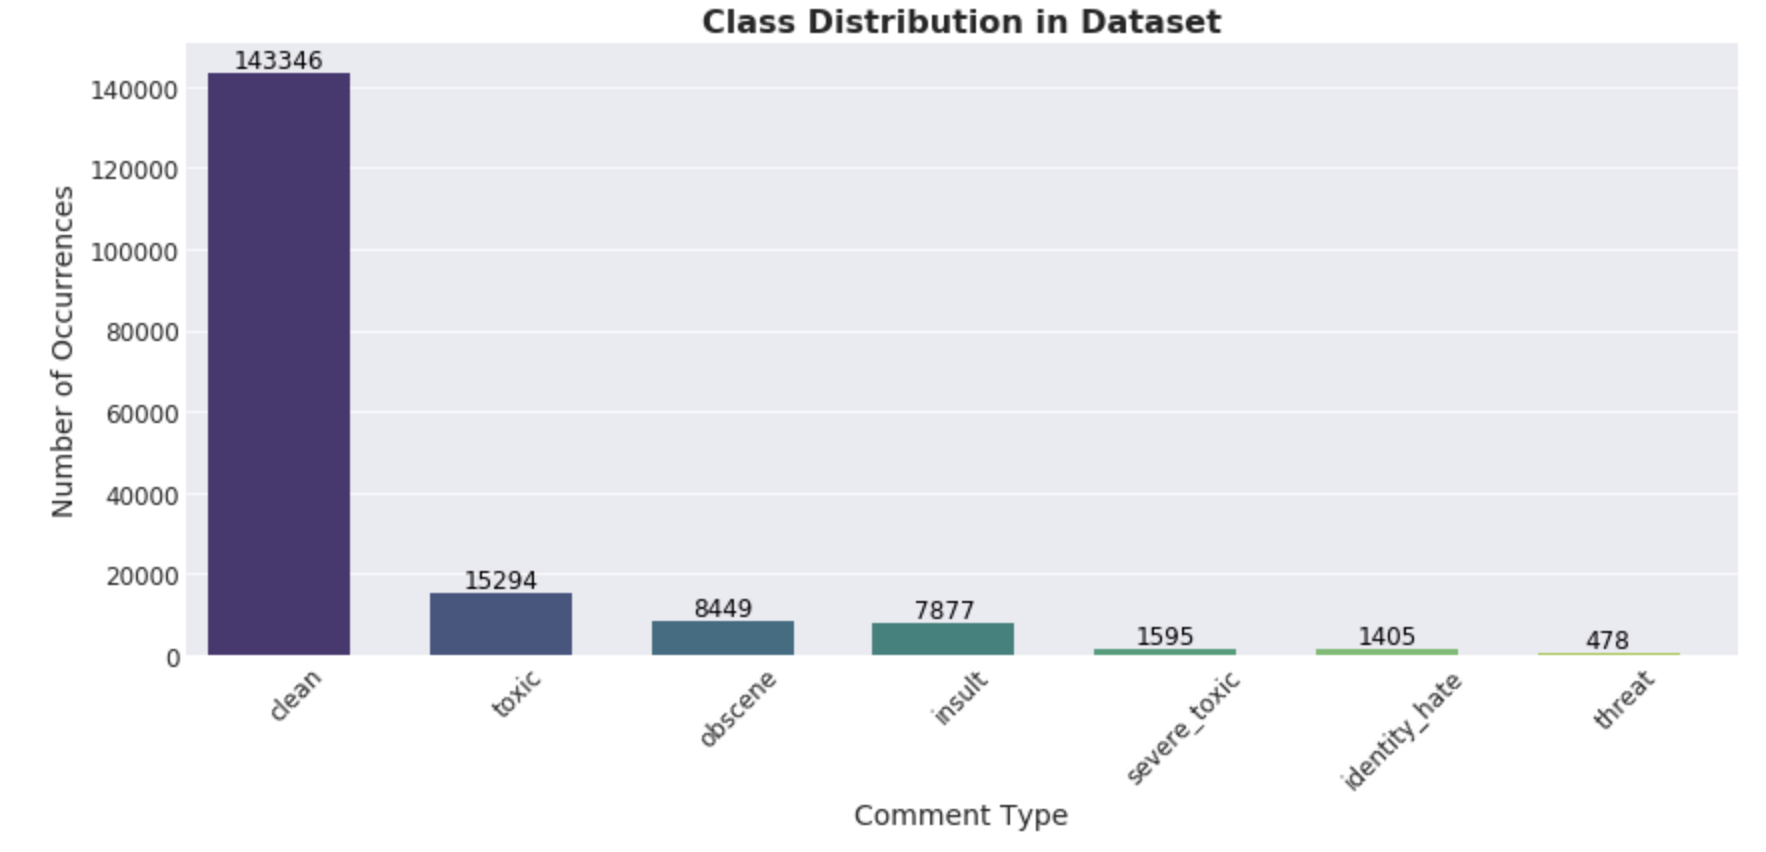
\includegraphics[width=7.5cm]{images/data_analysis/label_dist.png} }}%
    \qquad
    \subfloat[\centering Correlation between Toxicity Levels]{{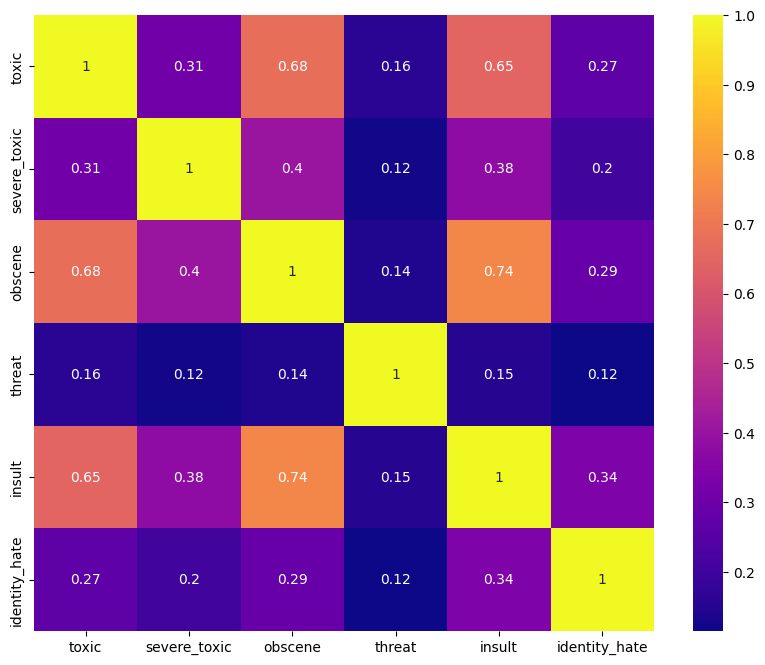
\includegraphics[width=5.5cm]{images/data_analysis/label_heatmap.png} }}%
    \qquad
    \subfloat[\centering Comment Length Density]{{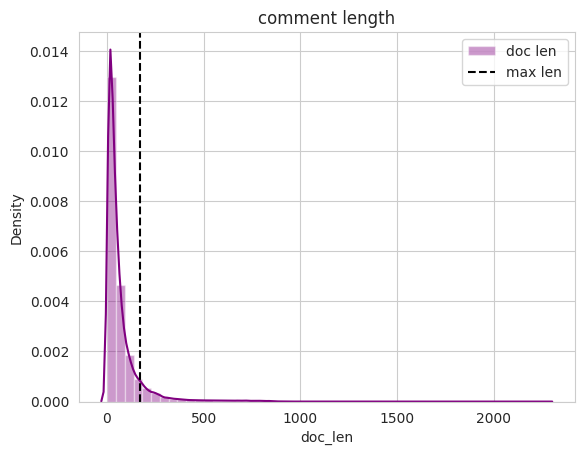
\includegraphics[width=5.5cm]{images/data_analysis/txt_len_density.png} }}%
    \caption{Dataset Analysis and Visualization}%
    \label{fig:dataset_analysis}
\end{figure}


\subsection{Dataset Distribution}
The dataset exhibits an imbalanced distribution with a significant majority of 'clean' comments (143,346 instances) (refer fig. \ref{fig:dataset_analysis}). The 'toxic' category follows with 15,294 instances, and subsequent categories like 'obscene' (8,449), 'insult' (7,877), 'severe\_toxic' (1,595), 'identity\_hate' (1,405), and 'threat' (478) are less frequent. Such an imbalance necessitates the use of specialized modeling techniques, such as resampling or class weighting, to ensure that minority classes are effectively represented.

\subsection{Correlation between Toxicity Labels}
Correlation analysis within the dataset indicates a strong positive correlation between 'toxic' and both 'obscene' (0.6765) and 'insult' (0.6475) categories, suggesting co-occurrence in comments. 'Severe\_toxic' shows moderate correlations with 'obscene' and 'insult,' whereas 'threat' and 'identity\_hate' demonstrate lower correlation with other categories, pointing towards the complexity of toxic language and the need for models capable of discerning the nuances between different types of toxicity.

\subsection{Comment Length Density} The density plot of comment lengths shows a peak at lower word counts, indicating that shorter comments are more prevalent. There is a noticeable decline in density as comment length increases, with the 'max\_len' parameter set to effectively encompass the majority of comments without excessive truncation. This parameter selection is instrumental for the LSTM model to perform optimally, given its reliance on sequential data for classification accuracy.